\chapter{Diskusjon}

\paragraph{}I dette kapittelet blir de ulike resultatene diskutert frem til en løsning. Dette kapittelet er en grundig undersøkelse, vurdering og forskning av alle løsninger. Her er målet å skape en objektiv diskusjon for å komme frem til en konkret og verdig løsning for problemet til Katoplast. 

\paragraph{}Ut i fra produktalternativene nevnt i punkt 4 ser vi at det finnes en rekke brukbare løsninger som kunne ha passet behovet til Katoplast. I disse produktalternativene finnes løsninger som skytjenester, Interne tjenester og hybrid tjenester. Ut ifra disse måtte prosjektet gjøre en vurdering av hvilke tjenester som skulle passe behovet til Katoplast best. 

\paragraph{} For at prosjektet skulle finne den beste løsningen til Katoplast valgte gruppen å lage en arbeidskravsanalyse opp i mot alle løsningene. I denne arbeidskravsanalysen tok prosjektet de samme arbeidskravene som gruppen hadde med i spørreundersøkelsen (3.1). Der ifra rangerer gruppen hvert av arbeidskravene fra en skala 1-100. Dette gjorde det lettere å kunne sammenligne med spørreundersøkelsen (3.1). Styrken med dette gjorde at gruppen kunne se hvilke løsning som ville treffe best etter behovet til Katoplast. Arbeidskravsanalysene som ble gjennomført ga en pekepinn på hvor prosjektet burde strekke seg.


\paragraph{} Tatt i betrakning er det noen arbeidskrav som veier opp mer enn andre. Når det kommer til sikkerhet, økonomi og nedetid er dette arbeidskrav som blir rangert høyere enn de andre arbeidskravene. Dette er de mest relevante arbeidskravene, og de har dermed størst betydning for prosjektets konklusjon.

\section{PC Hjelp AS}
\paragraph{} Det å finne en intern serverløsning for bedriften Katoplast var ikke den enkleste oppgaven. Leverandører av serverne var ikke åpne for å gi ut sine priser og løsninger. Etter mange samtaler med ulike leverandører over telefon og e-post, var det utfordrende å finne en løsning som var brukbar. PC Hjelp AS, arrangerte et møte med gruppen, hvor de presenterte sin løsning som kan være av interesse for Katoplast. 
\subsection{Fordeler}

\paragraph{} Interne servere kan ha kraftig sikkerhet dersom man er flinke til å oppdatere og vedlikeholde systemet. Tar man jevnlig backup og opprettholder backup-disken et annet sted enn der hvor serveren befinner seg, er det nesten umulig å miste data. Interne servere kan være kompliserte å drifte dersom man gjør dette selv. De fleste bedrifter benytter seg av IT-konsulenter for drift, men dette koster ofte en stor formue for få timers arbeid -derfor velger mange bedrifter heller å gjøre dette selv. Skulle noe av hardware gå i stykker er dette også utgifter som bedriften må betale.
\footnote{http://www.dwuser.com/education/content/why-you-need-a-testing-server-and-how-to-do-it/}


\paragraph{} Tilbudet prosjektet fikk tilsendt av PC Hjelpen AS var et langt mer pålitelig tilbud enn det Katoplast har fått tidligere. Hardware var langt mer skreddersydd og treffer langt bedre på de rammene Katoplast trenger. Den største fordelen med denne løsningen er at den letter på det økonomiske trykket som Katoplast opplever. Med en total pris på kun 25 530 kr blir kostnadene betraktelig mindre.

\paragraph{} I tilbudet som legges frem får Katoplast muligheten til å benytte seg av programvare og maskinvare som de allerede er kjent med. PC Hjelp tilbyr nemlig Windows Server 2012 som system. Med 2 x 1 terabyte harddisker får Katoplast mer enn nok lagringsplass til å lagre de verdifulle dataene de har, og samtidig ha nok plass til annen informasjon. Serveren som blir benyttet er Lenovo ThinkServer Xeon E3-1225v5. Dette er en kraftig maskin med 8 gigabyte RAM. Gruppen og PC Hjelpen AS ser ikke noe gevinst i å finne noe nyere software. Dette går kun utover budsjettet. 
\footnote{http://whatismyipaddress.com/localhost}

\paragraph{} Rundt konsulentarbeidet mener PC Hjelp as at de trenger mellom 4 til 7 timer for å implementere de nye serverene. PC Hjelpen tar 790kr i timen, noe som også er veldig rimelig opp mot vanlig konsulentarbeid. Arbeidet til konsulenten inkluderer klargjøring av ny datamaskin, installasjon av basis programmer og virusbeskyttelse. PC Hjelp AS ønsker også å ta en titt på situasjonen til Katoplast i dag for å kunne kartlegge server tilbudet mer effektivt. Dette er svært positivt med tanke på å finne den beste løsningen for Katoplast.

\paragraph{} 

\subsection{Ulemper}

\paragraph{} Ulempene med denne løsningen er at Katoplast først og fremst kommer til å fortsette å ha de administrative oppgavene som de gjerne ville slippe. De må da fortsette med drift og oppdateringer av serverne selv dersom de ikke ønsker å bruke innleide konsulenter. Et av ønskene til Katoplast var å unngå disse administrative oppgavene, men dette er problematisk å oppnå med en intern server som ikke gjør dette automatisk. \footnote{http://www.episerver.com/learn/resources/blog/udaiappa-ramachandran/the-pros-and-cons-of-cloud-storage/}

\paragraph{} En annen ulempe med løsningen er at den er lite fremtidsrettet. Det å ha servere på huset er en gammeldags metode som begynner å forsvinne. Flere og flere velger å gå for en mer fremtidsrettet løsning som en hybrid sky eller en vanlig sky tjeneste. Det er også slik at interne servere ofte opplever problemer med maskinvaren, noe som kan skape mer nedetid og feil som kan hemme arbeidet til bedriften. 

\section{Verdict}
\begin{figure}[H]
\centering
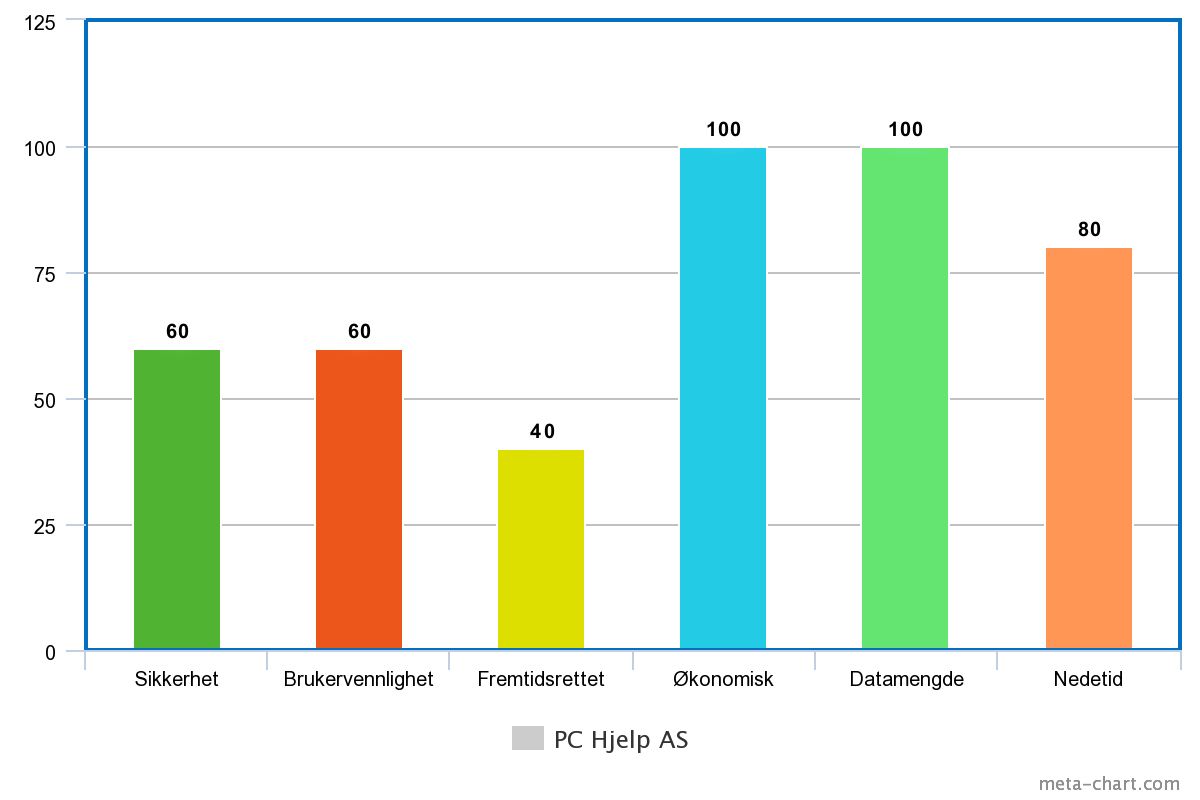
\includegraphics[width=6.5in]{Bilder/pchjelpchart.png}
\caption{Prosjektgruppens rangering av PC Hjelp sin løsning.}
\end{figure}

\section{Sky tjenester}

\subsection{Fordeler med Technet}
\paragraph{}Med sentraliserte IT-systemer i Technet sin skytjeneste, kan ny og krevende programvare settes i drift uten innkjøp av nye PCer og servere, eller behov for lokale oppgraderinger. Alle endringer skjer sentralt i Technet sin skytjeneste og den datakapasiteten som kreves blir produsert i en datasentral og bedriften kan planlegge når endringer skal skje og hvilke rettigheter brukerne skal tildeles i skytjenesten. Bedriften får en garantert oppetid på IT-løsningen, og har tilgang til egen IT-avdeling 24/7/365. Alle endringer skjer sentralt og den datakapasiteten som kreves blir produsert i en datasentral. 
\footnote{http://www.xn--skylsninger-jgb.no/skytjenester/}

\paragraph{} Nøkkelen til en problemfri IT-hverdag og et velfungerende IT-miljø, ligger i samspillet mellom hvert system, hver tjeneste og hver komponent. Brukerens IT-opplevelse avhenger av at alle komponentene, i en lang kjede, fungerer hver for seg og sammen med hverandre. Ved å ta et totalt ansvar kan Technet med sin skytjeneste sikre kvaliteten på komponentene som utgjør helheten. Resultatet er en skytjeneste som gir optimalisert IT-opplevelse for alle brukerne. Skulle et problem i skytjenesten oppstå har Technet ansvaret for alle potensielle feilkilder, enten dette gjelder nettverket, bredbåndslinjer, klienten eller applikasjonen. På den måten sikres i Technet sin skytjeneste effektiv feilsøking- og retting slik at man raskt kommer i gang med arbeidet igjen.


\subsection{Ulemper med Technet}
\paragraph{}Riktig skyløsning for bedriften er like siker som banken. Ulempen er den samme som fordelen- at du alltid er tilgjengelig. Dessuten finnes det så mange varianter av nettbrett og håndholdte enheter at det for en IT-avdeling kan være innviklet å sørge for ugjennomtrengelig sikkerhet. Ettersom bedriften må være avhengig av å måtte være koblet til internett, setter det også en avgrensing på dette. De fleste sky løsningene blir et mål for hackere. Dette setter enda større sikkerhetskrav til brukerne som har tilgang til enhetene. Det er lettere for en hacker å sende en falsk epost til en u-viten bruker på bedriften kontra å hacke technet sine servere. Den ene ulempen gruppen støtet på fra blant annet Technet og andre leverandører var at disse aktørene ønsket direkte kommunikasjon med Katoplast for å gi et pristilbud. Dette var noe som påvirket planleggingsfasen til prosjektgruppen.
\footnote{http://www.xn--skylsninger-jgb.no/om-skytjenester-fra-technet/}


\subsection{Fordeler med Azure}

\paragraph{}Det er mange positive sider med Azure løsningene til Microsoft. Skulle man trenge tilgang til dataene sine kan man lett få tak i disse ved bruk av en smart enhet. Det vil si at man kan ha tilgang på alle dataene sine når som helst, og hvor som helst uten begrensninger. Dette gjør det mulig for ansatte i bedrifter å kunne arbeide hvor som helst, til og med når de sitter hjemme. Man trenger altså ikke å sitte fysisk i lokalene til bedriften får å kunne utføre det arbeidet man er tilgitt. Med en slik fordel vil de ansatte ha muligheten til å arbeide mer effektivt, samtidig som de har mer tid dersom de ikke skulle klare å gjennomføre sine oppgaver på lokalene til bedriften. 
\footnote{https://azure.microsoft.com/nb-no/overview/what-is-azure/}

\paragraph{} En fordel med Azure er at den er brukervennlig. Det er Azure som tar seg av alt konsulentarbeid rundt serveren, og gir en essensiell og sikker måte å ta backup på. Ikke minst gir de muligheten til gjenoppretting med ekstern sikkerhetskopiering. Dette gjør at de sensitive opplysningene til en bedrift vil være helt sikre, selv om de skulle bli slettet eller filer skulle bli korrupte. Man har da muligheten til å gjenopprette slettede filer, eller tilbakestille arbeidet til en tid før det oppsto feil. Dette var en bekymring som Katoplast hadde, og som ønsket en løsning som tilbyr en sikker måte å gjenopprette data på.
\footnote{https://azure.microsoft.com/nb-no/services/site-recovery/}

\subsection{Ulemper med Azure}
\paragraph{} Det finnes i imidlertid en rekke ulemper med Azure. Sky løsninger er ofte et mål for hackere som ønsker å få tilgang til sensitive data og opplysninger. Microsoft som er et av verdens største organisasjoner er svært utsatt for slike angrep. Selv om Microsoft har sikkerhet av aller høyeste nivå, er det utfordrende å forebygge slike hacker angrep, og konsekvensene av angrepene er ofte store. Som følge av dette er det ofte slik at brukere og potensielle kunder holder seg til den gammeldagse metoden av å ha servere på huset. 
\footnote{https://www.scmagazineuk.com/microsoft-update-left-azure-linux-virtual-machines-open-to-hacking/article/575472/}

\paragraph{} En ulempe med Azure er at deres sky tjeneste befinner seg på et eksternt sted i verden som deres kunder ikke vet destinasjonen til. Et av Katoplast sine ønsker var at deres data og informasjon ikke skulle ligge hos en ekstern leverandør, ettersom de ikke ønsker at deres informasjon skal gå på avveie. Dette er en stor ulempe med Azure og med andre sky tjenester generelt, ettersom informasjonen lagres et annet sted en hos bedriften. Som følge av dette opplever Katoplast at deres informasjon ikke er sikker og kan i verste fall bli utnyttet av andre.
\footnote{http://www.biztechmagazine.com/article/2017/01/microsoft-warns-hacked-virtual-machines-are-very-real-threat}

\subsection{Azure Verdict}
\begin{figure}[H]
\centering
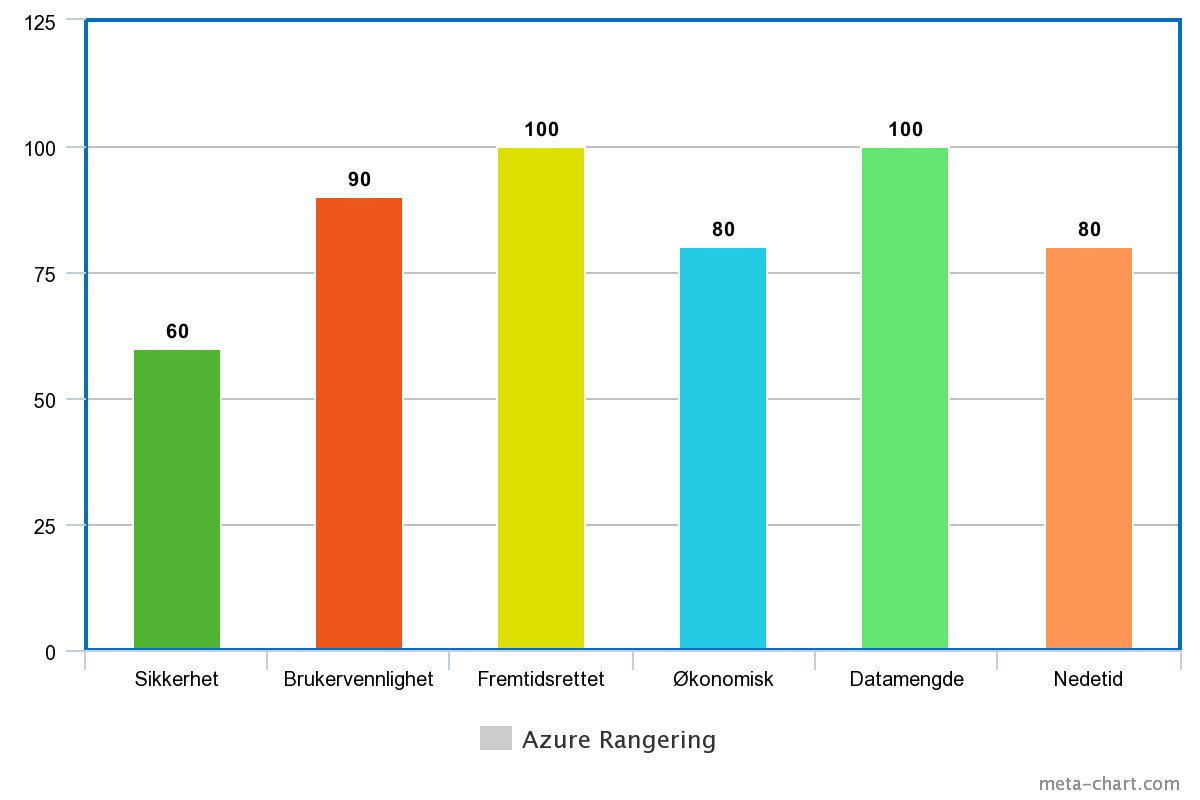
\includegraphics[width=6.5in]{Bilder/azurechart.png}
\caption{Prosjektgruppens rangering av Microsoft Azure.}
\end{figure}

\subsection{Fordeler med Amazon AWS}
\paragraph{} Det kan være en fordel å først og fremst beskrive hva Amazon sitt system tilbyr brukerne. Med Amazon Web Services ønsker Amazon å tilby en skytjeneste som er brukervennlig, fleksibel, kost-effektivt, pålitelig, skalerbar og sist men ikke minst sikker. Fordelen med AWS er at den tilbyr et hav av ulike tjenester og løsninger som brukere kan velge mellom. I tillegg tilbyr de fleksible betalingsmetoder hvor brukerne kun behøver å betale for det de bruker, ikke mer.
\footnote{https://aws.amazon.com/application-hosting/benefits/}

\paragraph{}Amazon AWS har en rekke fordeler. Som en ren skyløsning foregår ingenting internt, her blir det meste tatt hånd om. Derav er AWS veldig brukervennlig. De tilbyr også et bredt spekter av tjenester, som nevnt over, er det 70 forskjellige. De har også spredd rundt på jordkloden, i 16 forskjellige regioner. AWS er også ekstremt nøye på sikkerheten, og påstår at sikkerhet er deres høyeste prioritet. "We worked closely with the Amazon team to develop a security model, which we believe enables us to operate more securely in the public cloud than we can even in our data centers." (Alexander, 2015, AWS re:Invent)
\footnote{https://aws.amazon.com/security/}

\paragraph{} Også verdt å legge merke til, er at alle kontoer registrert i AWS blir lagt inn i en virtuell privat nettsky. Dette bidrar til å styrke sikkerheten rundt deres tjenester og ikke minst bidrar til å forebygge hacking og andre problemer. Det er også gunstig med AWS når selvstendige programvareskapere, slik som Microsoft, selger og inkluderer flere av sine egne produkter i systemet.
\footnote{https://aws.amazon.com/vpc/}

\subsection{Ulemper med Amazon AWS}
\paragraph{} Imidlertid, følger det en rekke ulemper med AWS. Serverene til AWS er alle virtuelle. Selv om klargjøringen er bedre, kan fortsatt ytelsen variere og det virtuelle vil ikke oppleves som like rent og stabilt som fysisk maskinvare. Læringskurven er samtidig bratt for større bedrifter. Dersom man har lite kunnskap innenfor å drifte eller benytte seg av virtuelle systemer, kan dette bli problematisk når man skal overføre arbeidet sitt fra fysiske maskiner til virtuelle systemer. 
\footnote{https://www.togglebox.com/blog/the-cons-of-working-with-amazon-web-services-aws/}
\footnote{https://npifinancial.com/blog/pros-and-cons-digging-into-amazon-web-services/}

\paragraph{} Det er også nødvendig å nevne, at flere små- og mellomstore bedrifter ikke får brukerstøtte og den veiledningen de trenger. Denne type nedprioriteringen er en omfattende ulempe, som kan føre til flere konsekvenser for en bedrift som ikke har den kunnskapen som kreves for drifting og oppsett av servere. Dette gjelder spesielt for Katoplast som, dersom de skulle bytte til en skyløsning, vil oppleve å måtte bruke tid og arbeid i å lære seg dette. Man vil naturligvis ha tilgang til brukerstøtte, men ikke i like stor grad som det andre leverandører tilbyr.
\footnote{https://www.liquidweb.com/blog/why-aws-is-bad-for-small-organizations-and-users/}


\paragraph{} Amazon sine tjenester har også opplevd avbrudd, hvor nedetiden har vart i flere timer. Dette er et problem som Katoplast ønsker å unngå, ettersom deres data og informasjon utgjør alt arbeid som utføres i bedriften. I Katoplast sitt tilfelle kan dette hemme arbeidet og kommunikasjonen innad bedriften og i verste fall føre til tap av penger.
\footnote{http://www.zdnet.com/article/how-amazon-web-services-crashed-and-rose-again/}
\footnote{http://www.geekwire.com/2017/amazon-explains-massive-aws-outage-says-employee-error-took-servers-offline-promises-changes/}

\subsection{Amazon AWS - Pris}
\paragraph{} Som nevnt i fordelene, tilbyr Amazon AWS en veldig fleksibel tjeneste, dette gjelder også prisen. Her betaler du for antall plass du bruker. Dette stiller jo til vesentlig fordel for et selskap som Katoplast som har tilgang til vesentlig mer plass enn de behøver. For kun 500GB arkivert over 40 år. Prisen til AWS avhenger av hvilken region du tilhører, hvis vi som eksempel velger London regionen, ser vi på en pris på rundt 0,0312 dollar pr GB, eller 0,3 NOK. Årlig koster dette cirka 12 000 NOK Som er en passende pris for løsningen. Dette er altså prisen på AWS S3, "simple storage service".
\footnote{https://npifinancial.com/blog/pros-and-cons-digging-into-amazon-web-services/}
\footnote{https://www.datastorageinc.com/blog/amazon-web-services-storage-pros-and-cons-for-document-management}

\section{StorSimple - Hybrid}
\subsection{Fordeler med StorSimple}
\paragraph{} StorSimple deles inn i 2 apparater hvor brukere kjøper et ønsket antall av virtuelle og fysiske apparater. Det finnes flere ulike modeller og hver av disse med deres egne fordeler. For Katoplast virket den beste løsningen å kjøpe en virtuell Modell 8010 server og en modell 8100 fysisk server for bedriften. Disse modellene utgjør til sammen litt over 1 Terabyte (TB) og utgjør mer enn nok lagringsplass for bedriften. Prisen på dette ligger på kr 11 834,25 månedlig kostnad, eller kr 142 011 årlig. Prisen er naturligvis varierende og Microsoft tillater flere kjøps alternativer for bedrifter.
\footnote{https://docs.microsoft.com/en-us/azure/storsimple/storsimple-technical-specifications-and-compliance}

\paragraph{} Det er en rekke ulike måter å gjennomføre et kjøp av en hybrid-tjeneste hos Microsoft. En fordel med Microsoft er at de tilbyr brukerne sine en rekke kjøps alternativer som kan lette litt på det økonomiske trykket som en bedrift kan oppleve. Med tanke på katoplast sin størrelse og hvilken økonomiske tilstand de er i, blir det beste valget å gå for Microsoft sitt "open-licensing program". Dette er et kjøps alternativ som Microsoft har utarbeidet med et sterkt fokus på små og mellom-store bedrifter. Mer detaljert, bedrifter med mellom 2 til 250 datamaskiner som ønsker å benytte seg av de tjenestene som Open Licensing Programmet tilbyr. 
\footnote{https://blogs.msdn.microsoft.com/mssmallbiz/2010/02/10/microsoft-open-license-basics-what-are-the-different-open-license-programs/}

\paragraph{} Innenfor Open Licensing Programmet tilbyr Microsoft en tjeneste for små bedrifter kalt "Open Value". Dette er et program anbefalt for små bedrifter. Løsningen tilbyr blant annet et fleksibelt brukergrensesnitt og kontroll over kjøpet og serverne som er bestilt. Kundene har muligheten til å overføre deres sensitive data og informasjon sakte, men sikkert over til Microsoft sin hybride plattform med den farten som er ønsket. Dette er avgjørende for å sikre en problemfri overføring fra interne servere til en hybrid løsning for Katoplast. Andre fordeler med Open Value inkluderer programvare oppgraderinger, hjelp med Microsoft lisenser, trening innenfor systemet og mer.
\footnote{https://www.microsoft.com/en-us/licensing/licensing-programs/open-license.aspx}

\paragraph{} I tillegg tilbyr Microsoft også online hjelp for bedrifter som skulle ønske eller trenge dette. Dette for å gjøre det lettere for mindre bedrifter som ikke har tilgang til dyre IT-konsulenter å forstå og sette opp deres server og abonnement. Med Microsoft sine dyktige og kunnskapsrike konsulenter, får Katoplast muligheten til å finne den beste avtalen for deres behov. 

\paragraph{} En sentral fordel med Microsoft sin Hybride Løsning er at det er enkelt å velge den datamengden man ønsker seg. Microsoft tillater brukerne å velge de serverne som skal ligge privat og de som skal ligge hos Microsoft. Brukerne får tilgang til en rekke modeller hvor de har muligheten til å velge akkurat hvor mange modeller de ønsker å ha og hvor hver av disse skal ligge. Man har muligheten til å velge akkurat de egenskapene man ønsker seg, uten at dette skal utgjøre noe problem. Datamengden er dermed akkurat slik brukerne ønsker det. 
\footnote{https://azure.microsoft.com/nb-no/pricing/calculator/}

\paragraph{} Løsningen er samtidig svært fremtidsrettet ettersom de hybride løsningene er en helt ny vei for Sky tjenestene. Microsoft fortsetter å sikte mot fremtiden og nylig har de introdusert sitt nye konsept "Nano Server" som hjelper til med å styrke infrastrukturen og sikkerheten til Microsoft sine servere og skyløsninger. Nano serverne danner samtidig en brukervennlig opplevelse når det kommer til kontrollering av servere.
\footnote{https://docs.microsoft.com/nb-no/azure/storsimple/storsimple-overview}

\paragraph{} Et kritisk mål for Katoplast var å få fjernet eller redusert store mengder av de administrative oppgavene som bedriften sliter med og som er svært tidkrevende. Nettopp dette har vært et betydelig fokus for Microsoft lenge, og med deres Windows PowerShell, får Katoplast løst deres problemer knyttet til administrative oppgaver. Med PowerShell blir mange av disse oppgavene automatisert, og Katoplast sparer massevis av tid og penger på å benytte seg av PowerShell. Bedriften har dermed muligheten til å legge sitt fokus på annet arbeid enn serverne.
\footnote{https://msdn.microsoft.com/en-us/powershell/mt173057.aspx}

\begin{figure}[H]
\centering
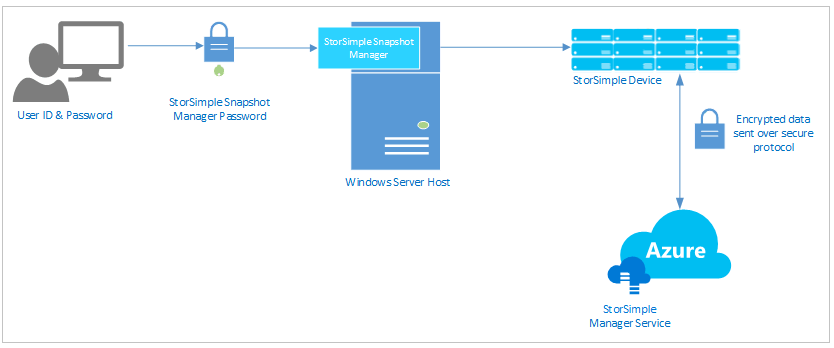
\includegraphics[width=6.5in]{Bilder/storsimple2.png}
\caption{Forenklet bilde av sikkerheten til StorSimple. (Dataencryption, 2016)}
\end{figure}

\paragraph{} Ofte er Microsoft og Sky tjenester koblet med svak sikkerhet. Mange brukere og kunder velger andre former for datalagring som følge av det faktum at Sky tjenester ikke er av den sikreste metoden å lagre data på. I midlertid, står en hybrid sky løsning for å løse dette. Med en slik tjeneste får Katoplast muligheten til å lagre sine sensitive data lokalt på huset, som kun de har tilgang til og som kun de har muligheten til å administrere. Med en slik mulighet blir mange av de bekymringene knyttet til sky lagring løst. Som Figur 5.1 viser så er StorSimple en svært beskyttet løsningen hvor det ikke bare kreves sterke og avanserte passord, men at data og informasjon først blir kryptert og skjult, før de sendes gjennom en sikret internett protokoll. Dette gjøres for å mest mulig sikre brukernes data fra angrep. 
\footnote{https://docs.microsoft.com/en-us/azure/storsimple/storsimple-security}

\subsection{Ulemper med StorSimple}
\paragraph{} StorSimple har mange funksjoner og tjenester ved seg som kan være til fordel for både små og store bedrifter. I midlertid, er ikke StorSimple et helt perfekt system og har en rekke ulemper ved seg. Med betraktning på Katoplast sine muligheter og begrensninger har gruppen kommet frem til en rekke ulemper som kan være interessant for Katoplast å vite og forstå.

\paragraph{} Først og fremst, et av de største ulempene med StorSimple, som med andre hybride løsninger, er at løsningen er dyr og utgjør en bemerkelsesverdig belastning for den økonomiske tilstanden til Katoplast. Med en prislapp på over 140 000 kr årlig, kan StorSimple utgjøre et problem for Katoplast sin økonomi. Selv om Microsoft har lagt et merkbart fokus for å muliggjøre sine løsninger for små bedrifter, er deres hybride skytjenester ikke av det billigste laget. Tjenestene er relative nye og er som følge av dette også kostbare. Det er mulig for Katoplast å få tilpasset løsningene og muligens få begrenset prisen. Foreløpig er prisen likevel høy.

\paragraph{} Den hybride løsningen til Microsoft fokuserer på å fikse mange av de bekymringene som brukere har knyttet til å lagre sensitiv data på et eksternt sted over internett. Likevel er det slik at Microsoft opplever mange former for datakriminalitet og de hybride løsningene kan oppleve å bli utsatt for slike angrep på lik linje med de vanlige sky løsningene. 
\footnote{http://www.eweek.com/cloud/microsoft-azure-flaw-exposed-rhel-virtual-machines-to-hacking-risk}

\paragraph{} En tredje ulempe med Microsoft er at de fra tid til annen opplever aggressive angrep fra enten hackere eller DDOS-angrep, som kan føre til at servere og ytelsen på Microsoft sine tjenester påvirkes. Som en konsekvens av dette kan tjenestene og serverne oppleve nedetid, og dette bør være en faktor som spiller inn dersom Katoplast skulle ønske å skifte over til Microsoft sin løsning. Likevel, er dette noe som skjer sjeldent og når det skjer så har det som oftest ikke alvorlige følger.
\footnote{http://www.networkworld.com/article/2224155/microsoft-subnet/microsoft-admits-to-being-hacked-too.html}

\subsection{StorSimple Verdict} 
\begin{figure}[H]
\centering
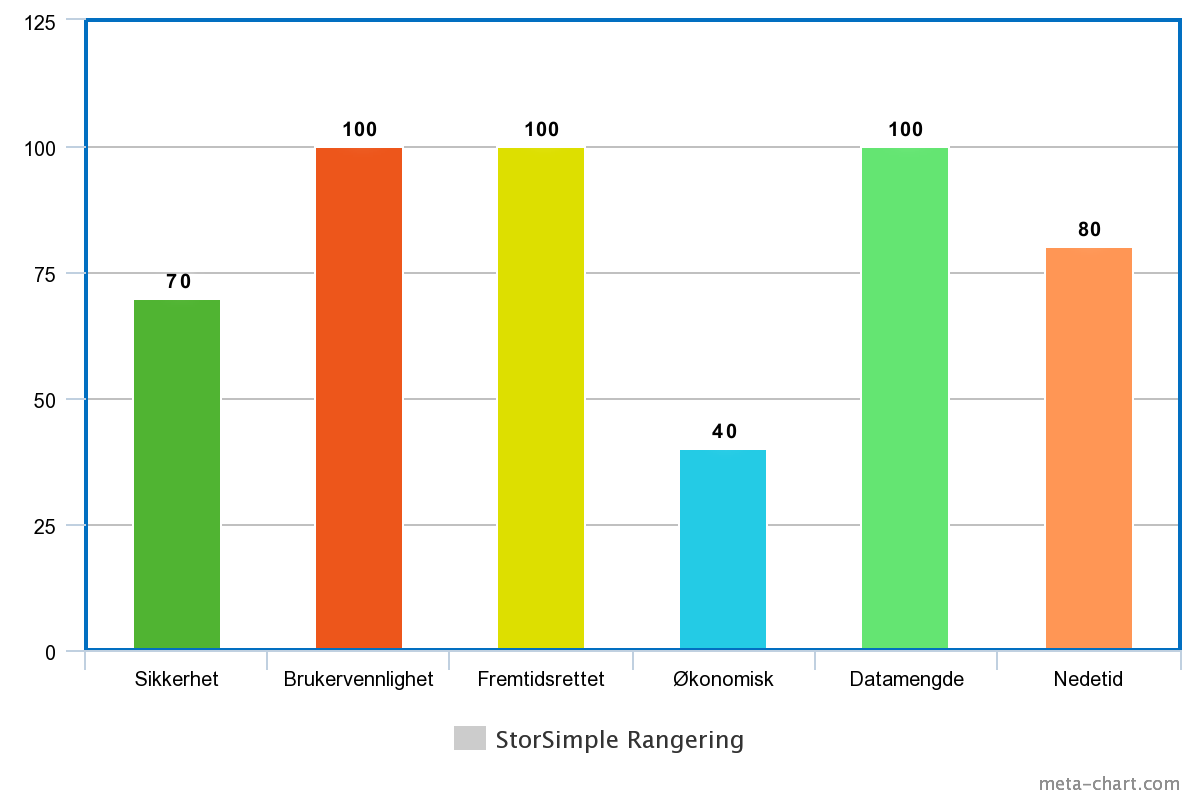
\includegraphics[width=6.5in]{Bilder/chart.png}
\caption{StorSimples rangering etter arbeidskravene.}
\end{figure}

\paragraph{} Dataene over tar i betraktning arbeidskravs analysen og gruppen rangerer StorSimple slik som figur 5.1 viser. Dette er gruppens vurdering av StorSimple ut i fra de kravene som er stilt og basert på resultatene og informasjonen som er samlet inn.

\section{VMware - Hybrid} 
\subsection{Fordeler med VMware}
\paragraph{} Som en av de senere organisasjonene til å introdusere Sky tjenester til omverdenen, har VMware fra tidligere etablert seg godt innenfor ytelse og pålitelighet. Med deres lange erfaring innenfor programvare utvikling som strekker seg helt fra 1998, har VMware håndtert overføring til å tilby skylagring av aller høyeste nivå på en positiv måte. Dette gjør VMware til en fordel når det gjelder fremtidig teknologi, ettersom de er raske med å etablere seg og har lang erfaring med programvareutvikling. 
\footnote{http://www.vmware.com/company.html}
\footnote{http://www.nytimes.com/2009/08/31/technology/business-computing/31virtual.html?pagewanted=2\&\_r=2\&partner=rss\&emc=rss}

\paragraph{} En vesentlig fordel med VMware er at de tilbyr brukerne sine å kontrollere alle tjenester gjennom deres  "vCloud Suite" platform. Dette gjør det lettere for brukere å administrere deres sky tjenester, samtidig som det gir forbedret kontroll over brukernes kjøp. Tjenesten assisterer også med å oppgradere programvare og verktøy, eller eventuelt nedgradere disse dersom en oppdatering skulle vise seg å være problematisk.
\footnote{http://www.vmware.com/products/vcloud-suite.html}

\paragraph{} VMware har, som tidligere nevnt, flere års erfaring med utvikling av programvare og applikasjoner. Med dette tilbyr de brukerne sine et bredt spekter av ressurser, funksjoner, verktøy og innebygde prosesser som hjelper med installasjon, oppsett og drifting av serverne, og ikke minst hjelpe kundene sine innenfor andre bruksområder. Samtidig, tar disse funksjonene seg også av de administrative oppgavene som Katoplast ofte føler tar en omfattende del av arbeidet når det gjelder deres servere. 
\footnote{http://www.vmware.com/products/vcloud-suite.html}

\paragraph{} Ikke minst, er disse programvarene en del av å opprettholde sikkerheten på den hybride løsningen. I motsetning til Microsoft så er ikke VMware i like stor grad under angrep av hackere. Dette gjør at VMware scorer høyere på sikkerhet enn det Microsoft gjør. I tillegg så er en hybrid løsning skapt for å sikre de sensitive opplysningene til en bedrift, ved at kun bedriften har tilgang til den private skyen.
\footnote{http://www.vmware.com/products.html}

\paragraph{} En positiv fordel med VMware sin løsning er at kundene som benytter seg av sitt kjøp, behøver kun å måtte betale for den dataen de benytter seg av og ikke noe mer. Dette er et omfattende steg mot en lettere økonomisk hverdag for katoplast når det gjelder servere. Med et slikt alternativ trenger ikke bedriften å bekymre seg for å måtte betale for ubrukte data. Katoplast betaler for 1,4 mer terabyte (TB) enn det de behøver, med deres nåværende løsning. Dette er overdrevent ettersom bedriften kun benytter seg av 500 gigabyte med lagringsplass!
\footnote{http://www.vmware.com/cloud-services/pricing-guide.html}

\begin{figure}[H]
\centering
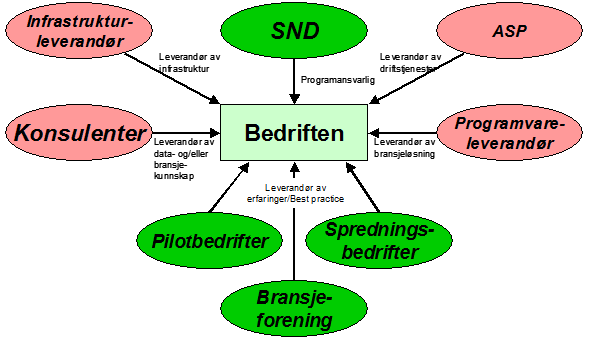
\includegraphics[width=6.5in]{Bilder/ss.png}
\caption{Nettverk av aktorer. (Christensen,2003, s.16)}
\end{figure}

\paragraph{} Som tidligere nevnt så tilbyr VMware ikke direkte sine løsninger til kunder, men gjør dette heller gjennom ulike partner nettverk, såkalte aktører. Hver av disse nettverkene bidrar med ressurser og verktøy til VMware, som hjelper med å danne de ulike løsningene som de tilbyr sine kunder. Samme opplegget kommer Katoplast til å oppleve når de må benytte seg av flere ulike aktører for deres server løsning. Fordelen med VMware og Microsoft er at disse aktørene deles heller i en, hvor leverandøren av løsningen også står ansvarlig for andre deler av prosessen. 
\footnote{http://www.tomsitpro.com/articles/hybrid-cloud-providers-comparison,2-841.html}
\footnote{https://www.vmware.com/partners.html}

\paragraph{} Figur 5.2 viser hvordan dette nettverket av aktører fungerer, og hvordan en bedrift får sine tjenester fra mange, ulike sider. VMware derimot inkluderer alle disse tjenestene i 1 pakke, hvor de samarbeider med ulike aktører, samt danner sine egne programmer. Dermed slipper Katoplast å måtte bekymre seg over å hyre inn egne konsulenter, programvare leverandører eller annet. De fleste hybride løsningene tilbyr dette i en helhetlig pakke som de gir til sine bedrifter, og med VMware sitt store partner nettverk er mulighetene enda større enn med andre løsninger.

\subsection{Ulemper med VMware}
\paragraph{} En ulempe med VMware er at deres forretningsmodell når det kommer til hybride løsninger er rotete. Dette gjør at kunder og brukere ofte ikke vet hva de egentlig betaler for og hva de egentlig får ut av de ulike alternativene som VMware tilbyr kundene sine. Dette kan påvirke installasjonen og oppdateringer av de hybride løsningene på en negativ måte. Det kan føre til at kunder benytter seg av feil programvare eller oppgraderer sine programmer uten å vite hva de egentlig gjør.
\footnote{http://marketrealist.com/2014/08/why-emc-vmware-and-pivotal-form-a-unique-business-model/}
\footnote{http://www.tomsitpro.com/articles/hybrid-cloud-providers-comparison,2-841.html}

\paragraph{} En annen ulempe med denne løsningen er at VMware ikke direkte er leverandøren av den hybride tjenesten. VMware er sponset av mange ulike nettverk som brukere må benytte seg av for å få tilgang til de hybride løsningene. Dette kan ofte føre til forvirring blant kunder om hvem de egentlig betaler til og hva de egentlig kjøper.
\footnote{https://www.vmware.com/partners/oem.html}

\paragraph{} Selv om VMware har lagt et betydelig fokus på brukervennlighet, føles det ikke alltid slik. Deres avanserte forretningsmodell og deres partner nettverk gjør det ikke lett for brukerne å forstå hvordan de skal gå frem med å kjøpe tjenestene og hvordan tjenestene helt fungerer. Spesielt når det gjelder kunder som ikke er eksperter innenfor IT-område. Selv om, mange av deres tjenester og produkter har et simplet brukergrensesnitt, påvirkes dette negativt av forretningsmodellen til VMware.

\paragraph{} Som med tidligere Hybride løsninger så er også VMware en relativt dyr løsning for en bedrift som Katoplast. Med en prislapp på litt over 81000 kr årlig, så er løsningen kostbar. Fordelene som følger med er enestående for bedriften, men overskygges av den høye prislappen.
\footnote{https://www.vmware.com/partners/partner-learning.html}

\subsection{VMware Verdict}
\begin{figure}[H]
\centering
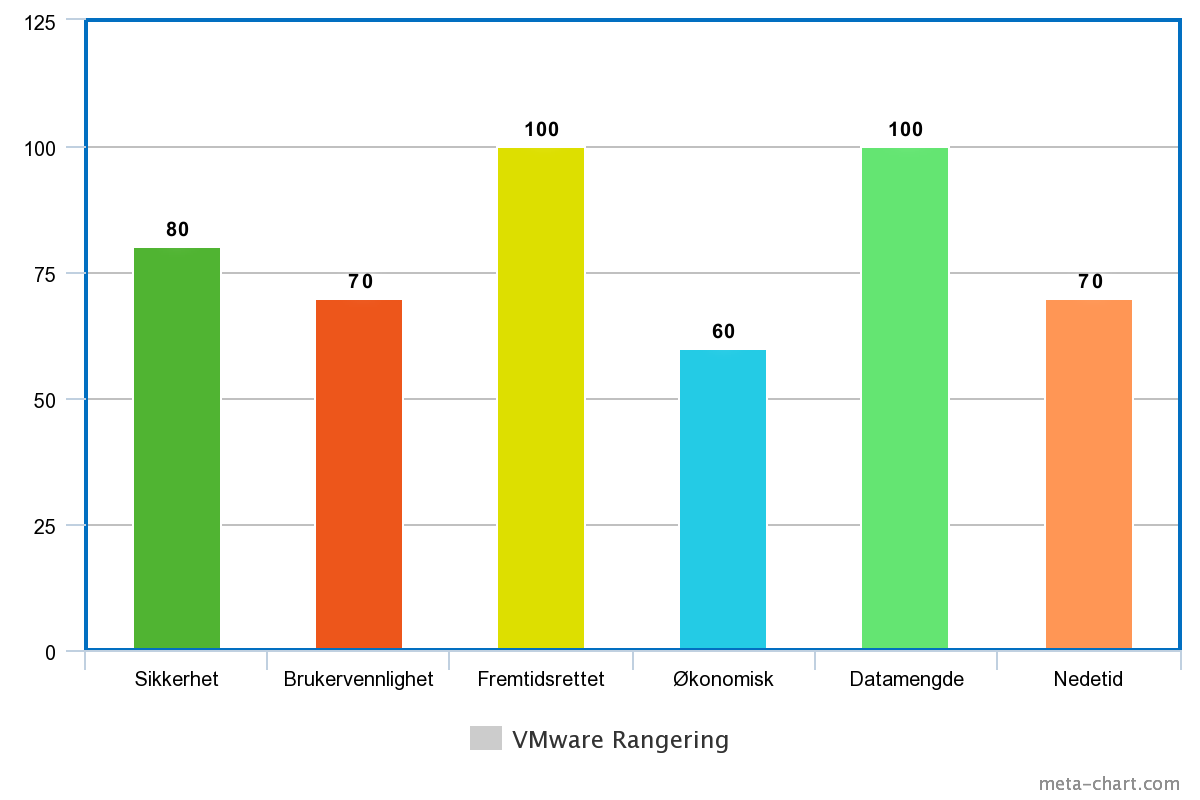
\includegraphics[width=6.5in]{Bilder/chart2.png}
\caption{VMware rangering etter arbeidskravene.}
\end{figure}

\paragraph{} Figure 5.2 viser hvordan prosjektgruppen rangerer VMware sin hybride løsning ut i fra de ulike arbeidskravene som har blitt stilt og ut i fra situasjonsanalysen som ble laget. Gruppen ønsker at Katoplast skal oppleve en helt ny hverdag med de nye hybride løsningene, hvor bedriften slipper å bekymre seg om sikkerheten og de administrative arbeidsoppgavene som må gjøres. VMware sin løsning er økonomisk sett billigere enn andre hybride løsninger.  Med en prislapp på cirka 81 000 kr årlig er løsningen fortsatt dyr, men mange hakk billigere enn andre løsninger. Det positive med VMware sin løsning derimot, er at den tar et godt steg inn i den hybride trenden som preger nye server løsninger. Dersom Katoplast skulle ønske å benytte seg av hybride løsninger er VMware sin løsning det beste startpunktet. 
